% PAKETE UND DOKUMENTKONFIGURATION
\documentclass[10pt, a4paper]{article}

% Encoding für Umlaute
\usepackage[utf8]{inputenc}

% Silbentrennung
\usepackage[ngerman]{babel}

% erweiterte Matheumgebungen
\usepackage{amsmath}

%
\usepackage{amsfonts}

%
\usepackage{amssymb}

% Einheiten setzen z.B. \SI{10}{\kilo\gram\meter\per\second\squared}
% Fehler: \SI{10 +- 0,2e-4}{\metre}
\usepackage{siunitx}
\sisetup{
  output-decimal-marker={,},
  separate-uncertainty
}

% Randbreiten
\usepackage[left=3cm,right=4cm,top=3cm,bottom=3cm,twoside]{geometry}

% Bilder einfügen
\usepackage{graphicx}

% Tiefe des Inhaltsverzeichnisses (Level: 1 sections, 2 subsections,
% 3 subsubsections)
\setcounter{tocdepth}{2}

% DOKUMENTINFORMATIONEN
\title{P422 \\ Rastertunnelmikroskopie}

\author{Christopher Deutsch\footnote{christopher.deutsch@uni-bonn.de} \and Christian Bespin\footnote{christian.bespin@uni-bonn.de}}

\date{\today}

\begin{document}
  
\maketitle

% DURCHFÜHRUNGSDATUM UND ASSISTENT
\begin{center}
\begin{tabular}{l r}
Durchführung: & 20./21. Oktober 2014 \\
Gruppe: & 2 $\alpha$ \\
Assistent: & Peter Klassen
\end{tabular}
\end{center}

% ZUSAMMENFASSUNG
\begin{abstract}
% Text
\end{abstract}

% INHALTSVERZEICHNIS
\tableofcontents
% Neue Seite nach TOC
\newpage

% INHALT VERSUCHSPROTOKOLL
\section{Grundlagen}

\subsection{Tunneleffekt und Tunnelstrom}
Der Tunneleffekt ist ein quantenmechanisches Phänomen, welches einem einlaufenden Teilchen der Energie $E$ erlaubt, eine klassisch unüberwindbare Potentialschwelle der Höhe $V_0 > E$ mit endlicher Wahrscheinlichkeit zu durchqueren.
Im Gegensatz zum klassischen Fall, bei dem das Teilchen am Potentialwall reflektiert wird, nimmt bei der quantenmechanischen Beschreibung das Betragsquadrat der Wellenfunktion $|\Psi|^2$ und damit die Aufenthaltswahrscheinlichkeitdichte des Teilchens, exponentiell mit der Eindringtiefe $s$ ab.

Dieser Effekt wird beim Rastertunnelmikroskop (RTM) ausgenutzt, indem eine Spannung zwischen dem zu untersuchenden, leitenden Objekt und der ebenfalls leitenden Spitze des RTM angelegt wird. Dadurch können Elektronen aus der Probe in die Spitze tunneln (oder umgekehrt), was zu einem Stromfluss $I_T$ führt.
Der Tunnelstrom für eine Potentialschwelle der mittleren Höhe $\Phi$ (für kleine Vorspannungen $U$ ist dies gegeben durch die Austrittsarbeit der Probe \cite{colton}) ist gegeben durch \cite{binning}:
\begin{equation}
  I_T \propto \exp(-\alpha \cdot \sqrt{\Phi} \cdot s) \quad \text{mit}\: \alpha = \SI{1,025}{\angstrom^{-1}\electronvolt^{-1/2}}
  \label{eq:tunnelstrom}
\end{equation}
also abhängig vom Abstand Spitze-Probe $s$, sowie von deren elektronischen Eigenschaften.
An Gleichung \ref{eq:tunnelstrom} erkennt man bereits die hohe Sensitivität auf Abstandsänderungen in der Größenordnung von einem \si{\angstrom}.
Aus diesem Grund ist das letzte Atom auf der Spitze maßgeblich für den gemessenen Tunnelstrom.

\subsection{Funktionsweise des Rastertunnelmikroskops}
\subsubsection{Aufbau}
\begin{figure}[h]
\centering
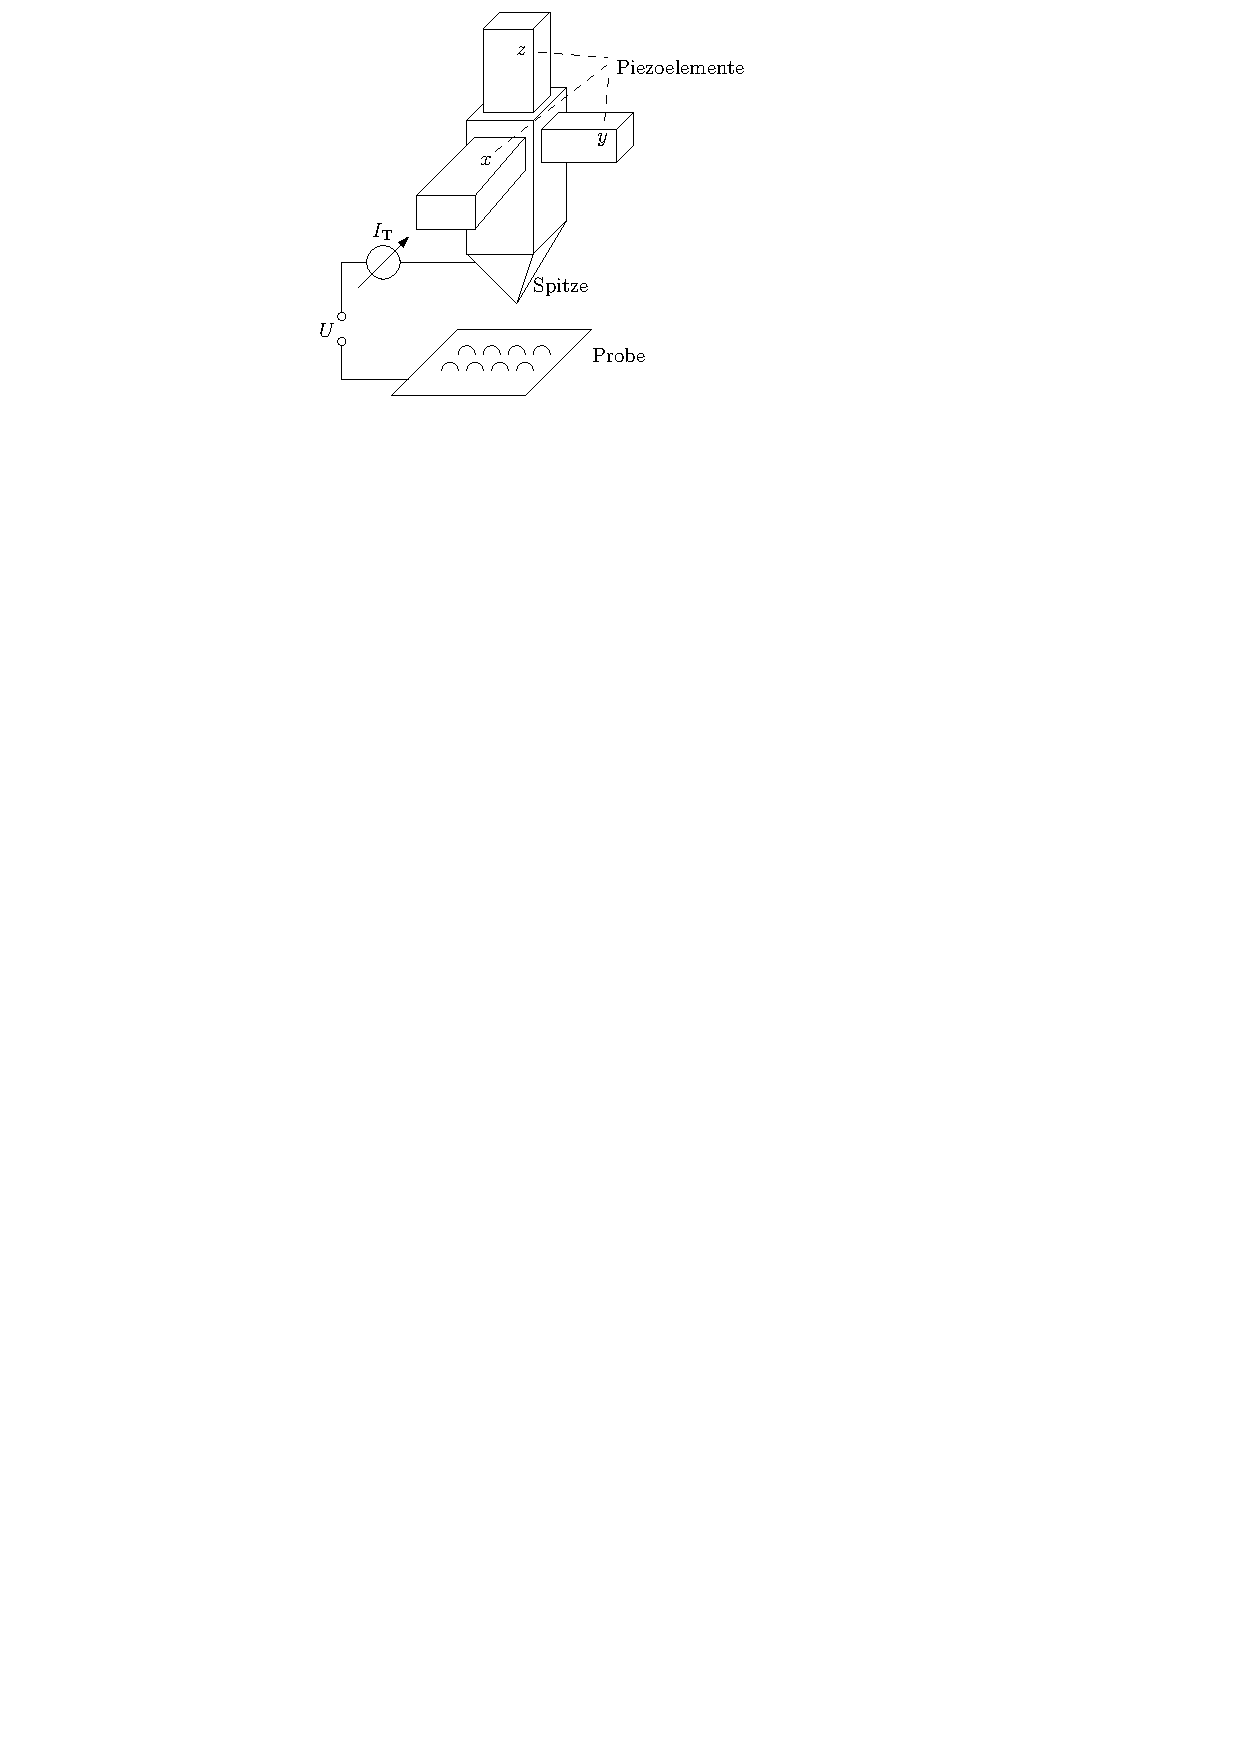
\includegraphics[width=0.5\textwidth]{./grafiken/rtm_aufbau.pdf}
\caption{schematischer Aufbau eines RTM mit Piezoelementen}
\label{fig:aufbau}
\end{figure}
Abbildung \ref{fig:aufbau} zeigt den schematischen Aufbau eines Rastertunnelmikroskops.
Dabei wird der Tunnelstrom $I_T$ gemessen und je nach Betriebsmodus (s.u.)  ausgewertet.
Die Piezoelemente dienen der Bewegung der Spitze in alle drei Raumrichtungen, wobei sie entweder automatisch gesteuert werden können (s. konstanter Tunnelstrom unter \ref{sec:betriebsmodi}) oder direkt gesteuert werden können zur manuellen Ausrichtung der Spitze.
\begin{itemize}
  \item Subatomare Auflösung -- Piezoeffekt
\end{itemize}
\subsubsection{Piezoeffekt}
In Elementarzellen mit nicht-inversionssymmetrischer Ladungsverteilung kann, beim Anlegen eines externen elektrischen Feldes, ein elektrisches Dipolmoment induziert werden.
Diese Polarisation führt zu einer Längenkontraktion/-ausdehnung der Elementarzelle aufgrund der Asymmetrie der Ladungsverteilung.
Dieser Effekt wird makroskopisch als Längenänderung eines piezoelektrischen Zylinders bei angelegter Spannung sichtbar.

\subsubsection{Betriebsmodi}
\label{sec:betriebsmodi}
Wir gehen im Folgenden davon aus, dass wir die Spannung zwischen Spitze und Probe in beiden Fällen konstant lassen.
Dann sind im Betrieb eines Rastertunnelmikroskops grundsätzlich zwei Betriebsmodi zu unterscheiden:
einmal wird der Tunnelstrom konstant gehalten, während im anderen Fall die Höhe der Spitze über der Probe konstant gehalten wird.
Im Fall des konstanten Tunnelstroms folgt die Spitze dem Profil der Probe.
Dies wird erreicht, indem der Tunnelstrom gemessen wird und durch eine Rückkopplungsschleife die Spitze so positioniert wird, dass der Tunnelstrom einen konstanten, vorgegebenen Wert annimmt.
Dafür sind die Piezoelemente notwendig, deren angelegte Spannung durch einen Regelkreis gesteuert wird.
Dessen Reaktionszeit sorgt dafür, dass das Verfahren im Vergleich zum Betriebsmodus mit konstanter Höhe deutlich langsamer ist, jedoch wird hier die Gefahr eines Zusammenstoßes von Spitze und Probe  unterbunden.

Im zweiten Fall wird die Spitze mit einer festgelegten und konstanten Höhe über die Probe bewegt und der Tunnelstrom gemessen.
Da seine Abhängigkeit von der elektronischen Struktur der Probe bekannt ist, lässt sich so ein Bild der Probe erstellen.
Da außer der Bewegung der Spitze in einer Ebene keine weiteren Regelungen notwendig sind, ist dieses Verfahren geeignet, um in kurzer Zeit Bilder der Probe zu erhalten, allerdings besteht dabei die Gefahr einer Kollision, bei dem die Spitze in die Probe fährt und dadurch zerstört wird.
Dieser Betriebsmodus ist also für flache Strukturen der Probe mit einer durchschnittlichen Höhe kleiner als der Abstand Probe-Spitze geeignet \cite{colton}.
Da es praktisch kaum möglich ist, vertikale Verschiebungen auszuschließen und die Probe nicht immer parallel zur horizontalen Bewegung der Spitze ausgerichtet ist, wird auch hier eine Rückkopplungsschleife, wie oben erklärt, verwendet, allerdings mit einer geringen Empfindlichkeit. Dadurch ist sichergestellt, dass die Spitze nicht auf schnelle Änderungen des Tunnelstroms reagiert, aber langfristig eine vorgegebene Höhe über der Probe (auch wenn diese gegen die horizontale Bewegungsebene der Spitze geneigt ist) erreicht wird.
 
\begin{itemize}
  \item Konstanter Tunnelstrom (Rückkopplungsschleife und deren Reaktionszeit, proportional zum Probenprofil)
  \item Konstante Höhe (Tunnelstrom wird aufgezeichnet, proportional zur elektronischen Struktur, \emph{Crash}, schnell)
\end{itemize}

\subsubsection{Regelkreis}
\subsubsection{Auflösungsvermögen}

\subsection{Spitzenherstellung}
Um ein möglichst hohes Auflösungsvermögen zu erreichen, ist eine dünne Spitze (idealerweise ein einzelnes Atom) nötig. (Ätzen steht in \cite{colton})
Im Folgenden werden die im Versuch verwendeten Spitzenherstellungsmethoden diskutiert.

\subsubsection{Reißen von Platin-Iridium Spitzen}
Die Spitze eines Platin-Iridium Drahtes wird mit einem flach angesetzten Seitenschneider abgerissen. (Oxidiert nicht)

\subsubsection{Ätzen von Wolfram Spitzen}
An Luft bildet Wolfram schnell eine nichtleitende Oxidschicht, die die Spitzenqualität negativ beeinflusst.
Ein Wolframdraht wird in einer Kalilauge (KOH 2 M (2 \si{\mol\per\litre})) eingetaucht. Im Elektrolyt befindet sich um diesen eine ringförmige Elektrode, welche die Ätzwirkung auf einen kleinen Bereich des Drahtes einschränkt.

\subsection{Kristallstruktur von Graphit}
\begin{figure}[h]
  \centering
  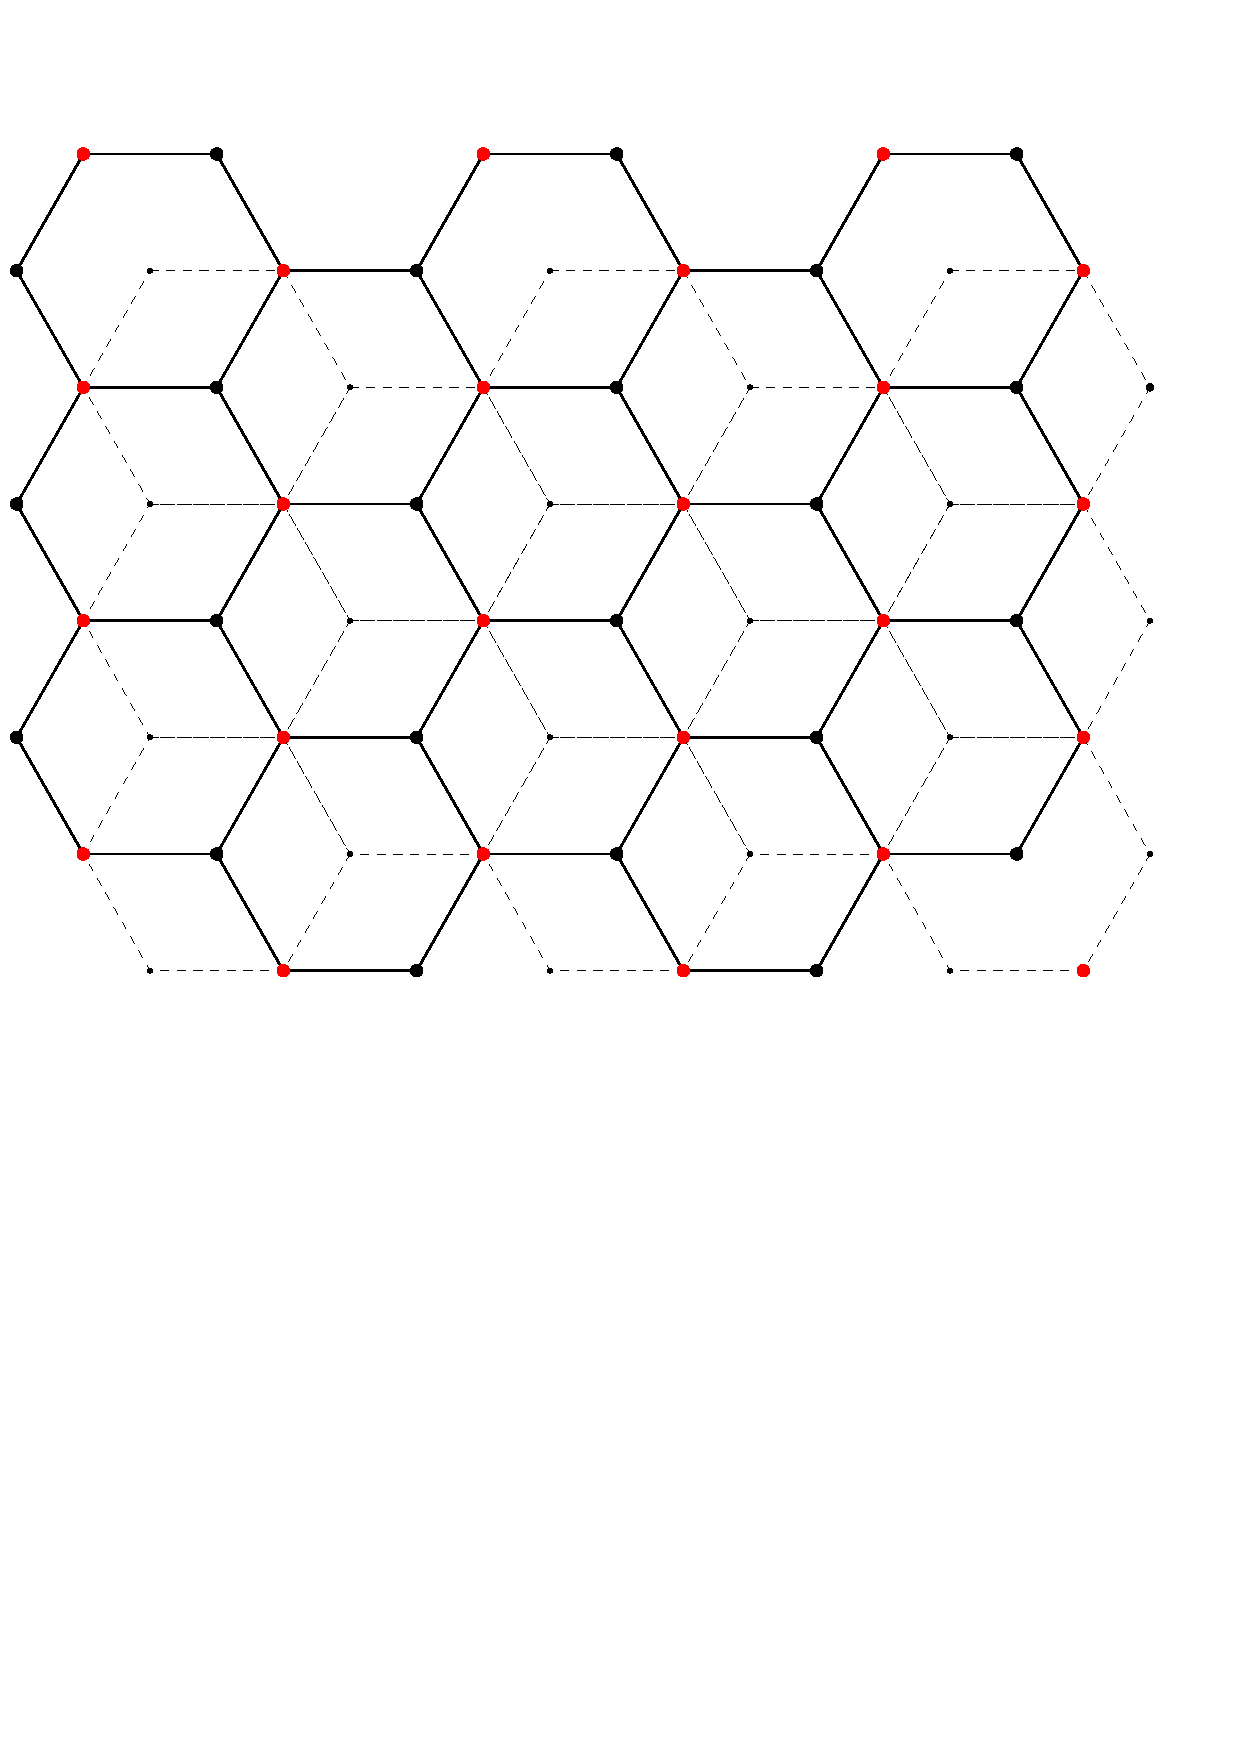
\includegraphics[width=0.6\textwidth]{grafiken/graphit.pdf}
  \caption{Versatz der Graphen-Ebenen in Graphit. Kohlenstoffatome in rot überlappen in den beiden obersten Ebenen}
\end{figure}
Graphit besteht aus geschichteten Ebenen von Kohlenstoff, welcher eine hexagonale Ringstruktur aufweist. 

\subsection{Verwandte Rastermethoden}
\begin{itemize}
  \item \textbf{Rasterkraftmikroskopie:} Um nicht-leitende Oberflächen zu untersuchen ist die Rastertunnelmikroskopie ungeeignet.
  Stattdessen nutzt man die interatomaren Kräfte zwischen dem Objekt und einer Blattfeder mit dünner Spitze aus, um aus deren Auslenkung das Profil der Oberfläche zu bestimmen.
  Ähnlich zum RTM gibt es im Kontaktbetrieb des Rasterkraftmikroskops zwei typische Betriebsmodi:
  \begin{itemize}
  \item[--] konstante Kraft: Eine Rückkopplungsschleife zwischen Auslenkungsmessung und Höheneinstellung sorgt dafür, dass die Auslenkung und damit die Kraft konstant gehalten wird.
  So ist das Profil des Objektes gegeben durch die Blattfederhöhe.
  \item[--] konstante Höhe: Die Höheneinstellung bleibt unverändert und das Profil des Objektes ist gegeben durch die Auslenkung der Feder.
  \end{itemize}
  Es gibt noch weitere Betriebsmodi auf die hier nicht weiter eingegangen wird.
  \item \textbf{Rasterelektronenmikroskopie:} Ein gebündelter Elektronenstrahl wird über ein Objekt gerastert.
  Die dabei entstehenden gestreuten Elektronen, Sekundärelektronen, Bremsstrahlung etc. können über Detektoren eine Abbildung des Objekt reproduzieren.
\end{itemize}

\section{Versuchsdurchführung}

\section{Messdaten}

\section{Auswertung}

\section{Diskussion}

\section{Zusammenfassung}

% BIBLIOGRAPHIE

% Maximale Anzahl der Einträge in Klammer
% Zitieren mit \cite{lamport94}
\begin{thebibliography}{9}

% Beispiel
\bibitem{binning}
  G. Binning et al.,
  \emph{Surface Studies by Scanning Tunneling Microscopy},
  Phys. Rev. Lett. 49, 57 (1982).

\bibitem{colton}
  R. J. Colton, A. Engel, J. E. Frommer et al.,
  \emph{Procedures in Scanning Probe Microscopies},
  John Wiley 1998.
  
\end{thebibliography}

\end{document}
